\begin{flushright} {\tiny {\color{gray} python\_codes/fieldstone\_114/text.tex}} \end{flushright}

%\lstinputlisting[language=bash,basicstyle=\small]{python_codes/fieldstone_114/keywords}

\begin{center}
\fbox{\textbf{\huge \color{teal} P}}
Codes at \url{https://github.com/cedrict/fieldstone/tree/master/python_codes/fieldstone_114}
\end{center}

\par\noindent\rule{\textwidth}{0.4pt}

{\sl This fieldstone was developed in collaboration with W. Klessens}. \index{contributors}{W. Klessens}

\par\noindent\rule{\textwidth}{0.4pt}
%%%%%%%%%%%%%%%%%%%%%%%%%%%%%%%%%%%%%%%%%%%%%%%%%%%%%%%%%%%%%%%%%%%%%%%%%%%%%%%%%%%%%%%%%%%%%%

This \stone is inspired by \textcite{bakp14} (2014).
The setup is as follows:

\begin{center}
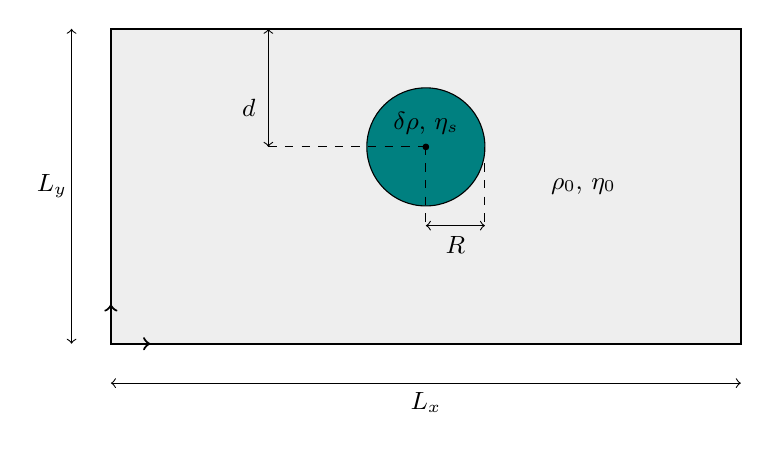
\begin{tikzpicture}
%\draw[step=0.5cm,gray,very thin] (0,0) grid (10,6); %background grid
\draw[fill=gray!63,gray!13](1,1) rectangle (9,5);
\draw[thick] (1,1) -- (9,1) -- (9,5) -- (1,5) -- cycle; %top
\draw[black,fill=teal] (5,3.5)   circle (0.75cm);
\draw[thick,->] (1,1) -- (1.5,1); 
\draw[thick,->] (1,1) -- (1,1.5); 
\draw[black,fill=black] (5,3.5)   circle (1pt);
\draw[thin,<->] (0.5,1) -- (0.5,5); 
\draw[thin,<->] (1,0.5) -- (9,0.5); 
\draw[thin,<->] (3,3.5) -- (3,5); 
\draw[thin,<->] (5,2.5) -- (5.75,2.5); 
\node[] at (5,0.25) {\small $L_x$};
\node[] at (0.25,3) {\small $L_y$};
\node[] at (2.75,4) {\small $d$};
\node[] at (5.375,2.25) {\small $R$};
\draw[dashed,thin] (3,3.5)--(5,3.5);
\draw[dashed,thin] (5,3.5)--(5,2.5);
\draw[dashed,thin] (5.75,3.5)--(5.75,2.5);
\node[] at (7,3) {\small $\rho_0$, $\eta_0$};
\node[] at (5,3.8) {\small $\delta\rho$, $\eta_s$};
\end{tikzpicture}
\end{center}

When the sphere is lighter than its surrounding it goes up and creates a 
divergent flow at the surface. As explained in \textcite{bakp14} an analytical 
solution exists for the horizontal component of the velocity at the surface in 3D. 
Also, the lower density of the sphere (or rather the density difference $\delta\rho$
between the sphere and its surrounding) yields a gravity field 
above the sphere that is lower and for which an analytical solution exists too.

Assuming we have determined what the depth of the sphere is (and assuming that 
it is rigid by taking its viscosity $\eta_s >> \eta_0$), then the two main 
+unknowns are its density difference $\delta \rho$ with regard to the surrounding mantle
and its radius $R$. 

To start with, we can compute analytically the gravity and velocity that a 
$\delta\rho^\dag=-300$ and $R^\dag=50~\si{\km}$ disc generates at the surface of the model,
write a simple inversion code which would operate in the $(R,\delta\rho)$-space 
and automatically looks for the real values of the sphere by computing a gravity misfit $\xi_g$ 
and velocity misfit $\xi_v$ and using these quantities to zero-in on the correct values 
of $\delta \rho$ and $R$.


Three ideas:

- axisymmetric

- full 3D

- try JIT? julia?


%--------------------------------------------------------
\subsection*{gravity forward model - analytical solution}

We consider a circular inclusion at half the 2D domain of 
$1000~\si{\km}$ in $x$- and $500~\si{\km}$ in $y$-direction. 
Because of the evident symmetry of the problem we restrict the 
calculations to the right half of the domain so that now it 
is a square of size $L_x=L_y=500~\si{\km}$ and the sphere is 
at coordinates $(x_c,y_c)=(0,Ly/2)$.

In the case of a disc, the gravity in the $x,y-$plane is given by 
\[
\vec{g}(x,y) = {\cal G} \frac{\pi R^2 \delta\rho}{(x-x_c)^2+(y-y_c)^2} 
\left(
\begin{array}{c}
x-x_c \\
y-y_c
\end{array}
\right)
\]
In the case of a sphere, 
\[
\vec{g}(x,y,z) = {\cal G} \frac{\pi R^2 \delta\rho}{(x-x_c)^2+(y-y_c)^2+(z-z_c)^2} 
\left(
\begin{array}{c}
x-x_c \\
y-y_c \\
z-z_c 
\end{array}
\right)
\]
Gravity is computed by transforming the integral 
\[
\vec{g}(x,y) = \iiint_V {\cal G} \frac{\rho(x',y',z')}{ (x-x')^2+(y-y')^2+(z-z')^2    } dx'dy'dz'
\]
over the domain by a sum of elemental 
integrals which are then computed by means of the same quadrature as the FE matrix. 
Since half the disk is missing, we on-the-fly take the missing half into account by 
mirroring the quadrature points and adding their contribution. 

Because we are only interested in the gravity signal generated by the disc/sphere, 
a boolean array {\tt elt\_in\_sphere} is created and set to true for those elements
for which at least one quadrature point is inside the sphere. This array is then used
to target the contribution of the elements 'inside' the sphere. 



%--------------------------------------------------------
\subsection*{Stokes forward model - analytical solution}

The surface velocity signal of a rising sphere is computed in Appendix~A of \textcite{bakp14} (2014).
It is based on \textcite{bren61} (1961), \textcite{stje26} (1926) and \textcite{pacy05} (2005). See also 
\textcite{burg16} (1916). The solution is only available in 3D with axisymmetric geometry. 
The analytical expression is rather complex and in order to keep simple for now, we
will use a different reference velocity quantity to carry out the inversion. 
In the folder {\tt reference\_code} a modified version of \stone~2 is placed. 
It computes the velocity field for the reference case
at a 150x150 resolution. The root mean square velocity 
$\upnu_{rms}=7.740432578645655e-10~\si{\meter\per\second}$ 
will serve as our reference value to drive the inversion.

\begin{center}
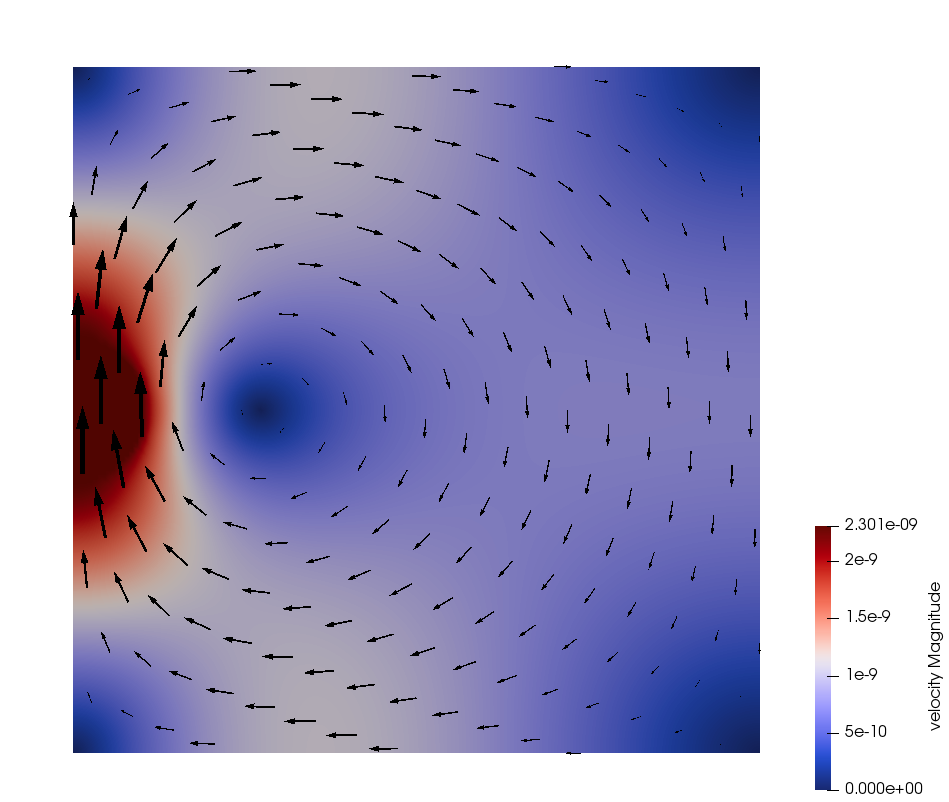
\includegraphics[width=6cm]{python_codes/fieldstone_114/reference_code/vel}
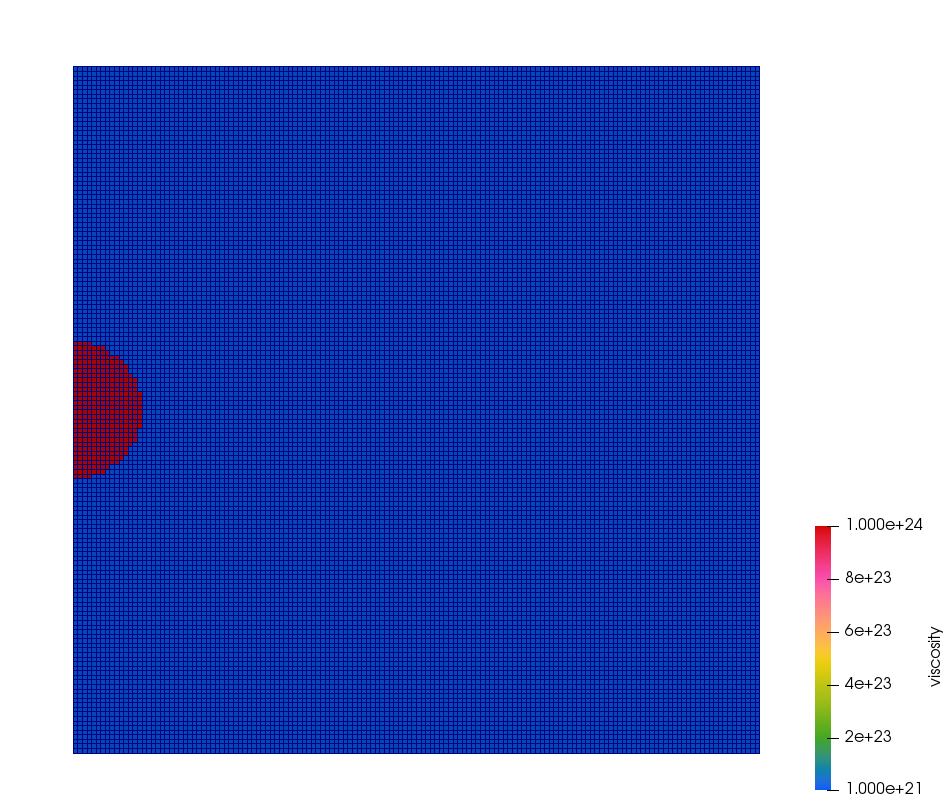
\includegraphics[width=6cm]{python_codes/fieldstone_114/reference_code/eta}\\
{\captionfont Sphere radius is $R=50~\si{\km}$, $\rho_m=3000$, $\delta\rho=-300$, $\eta^\star=10^3$.}
\end{center}

%--------------------------------------------------------
\subsection*{The code}

In order to produce a reasonably fast Stokes solver the code relies on 
the $Q_1\times P_0$ element with a penalty approach (see for example \stone~01).
The Cartesian domain is overlain with a mesh counting $nel_x\times nel_y=nel$
elements which are all square, so that the Jacobian of the transformation
between global and local coordinates is diagonal. Its value has been 
hard-wired in the code so as to save time. 
The entire Stokes solver + gravity calculator is inserted into a single function
{\tt compute\_misfits} in the {\pythonfile forward.py} file.

Note that depending on the mesh resolution a call to the function will take betweem 1s 
(50x50) 2.5s (64x64), and 8s (100x100). 

%--------------------------------------------------------
\subsection*{Inversion}

The first inversion code {\pythonfile driver1.py} is very simple. The user defines the bounds of the 
parameter space, i.e. $\delta\rho_{min}$, $\delta\rho_{max}$, $R_{min}$ and $R_{max}$.
Then a regular grid composed of $n_{\delta\rho} \times n_{R}$ is used to compute 
both misfits $\xi_g$ and $\xi_v$ at each node of the grid and these are 
exported in a vtu file. No refinement or clever search takes place. 

\begin{center}
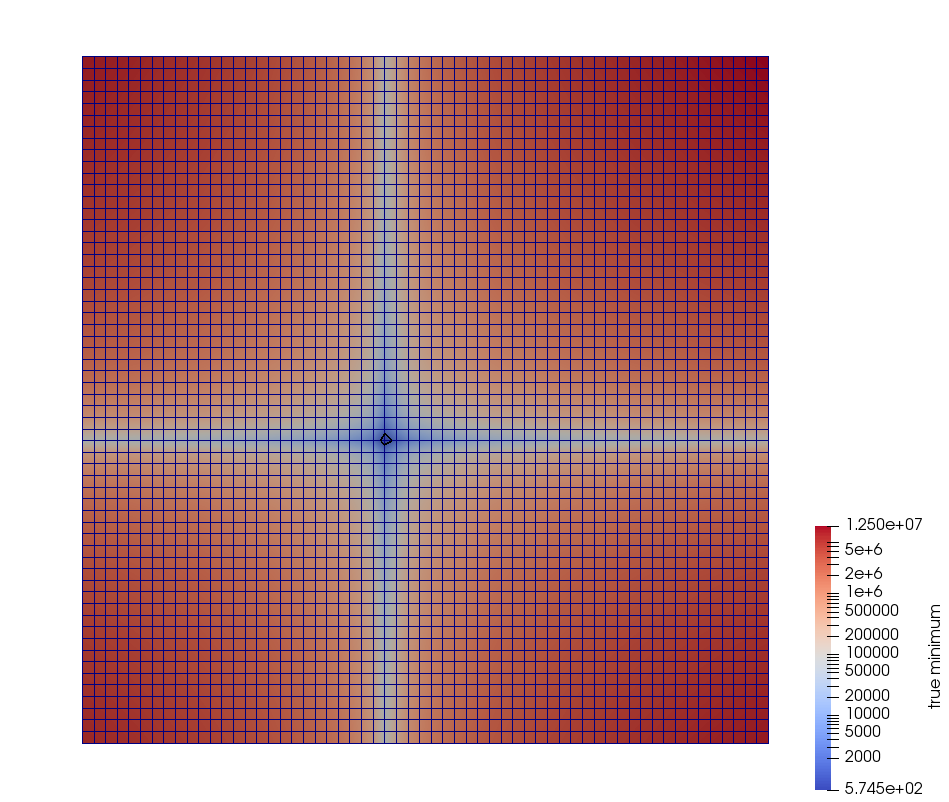
\includegraphics[width=5.7cm]{python_codes/fieldstone_114/results/min}
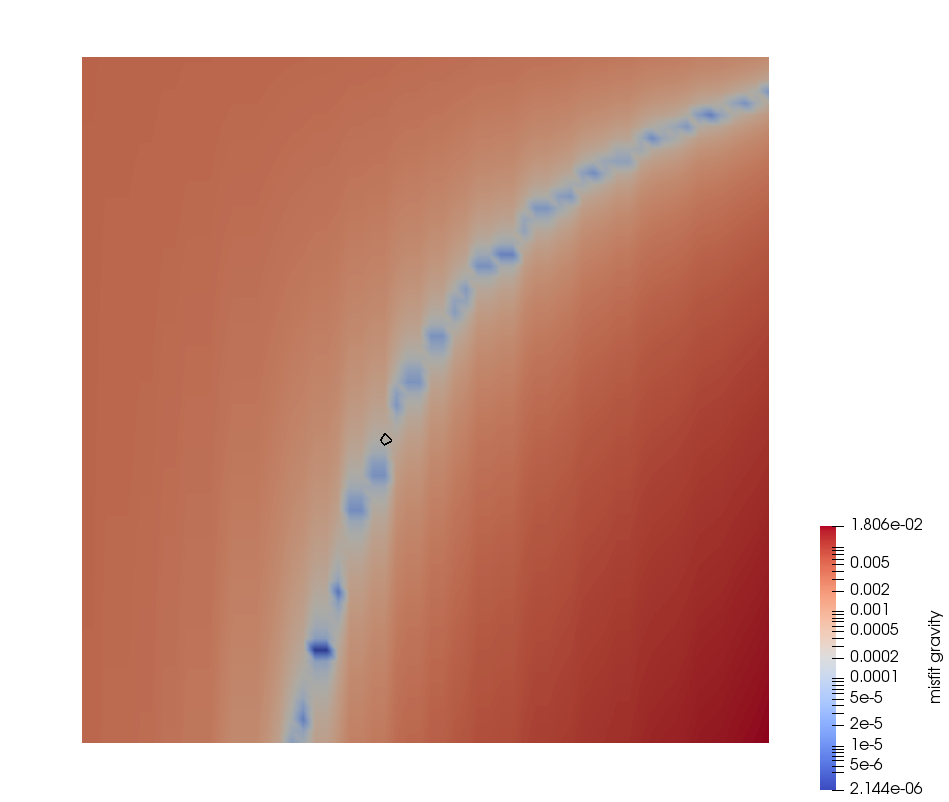
\includegraphics[width=5.7cm]{python_codes/fieldstone_114/results/mg}
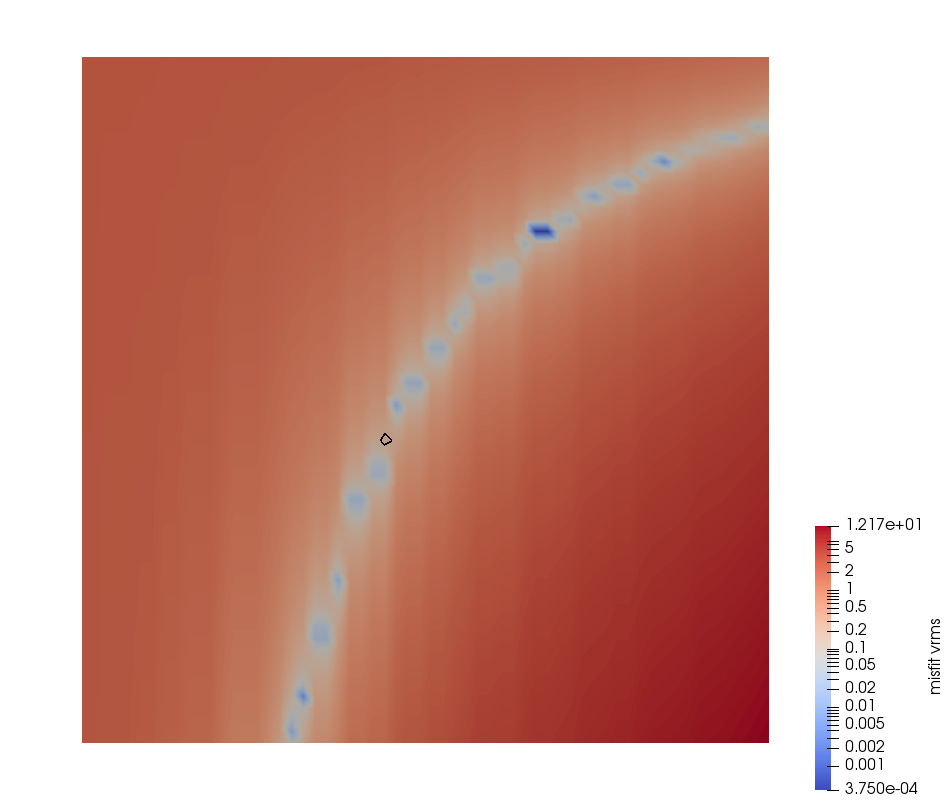
\includegraphics[width=5.7cm]{python_codes/fieldstone_114/results/mv}\\
{\captionfont horizontal axis is radius $R$, vertical axis is $\delta\rho$. 60x60 points. about 2.5h.
Left: location of the true minimum, i.e. the reference model; Middle: gravity misfit; Right: vrms misfit.} 
\end{center}




